%%%%%%%%%%%%%%%%%%%%%%%%
%
% $Autor: Sadegh Naderi $
% $Datum: 2023-02-11  $
% $Short Description: The results obtained by the model and the board $
% $Directory: ML23-01-Keyword-Spotting-with-an-Arduino-Nano-33-BLE-Sense\report\Contents\en\DocumentationDevelopment .tex $
% $Version: 1.0 $
% $Review by: Sadegh Naderi $
% $Review date: 2023-02-11 $
%
%%%%%%%%%%%%%%%%%%%%%%%%


\chapter{Results}


\section{Data Transformation}

To convert audio to a spectrogram, one-second audio snippets are analyzed in a loop, applying fast Fourier transform (FFT) to each 30-millisecond segment with a 20-millisecond overlap. This process produces a 2D array representing the entire audio sample (See Figure \ref{fig:audioWaveSpectrogramYes}). This 2D array, commonly known as a spectrogram, captures the intensity of different frequency components across time. The spectrogram is then fed to the CNN model.

\begin{figure}[h!]
	\centering
	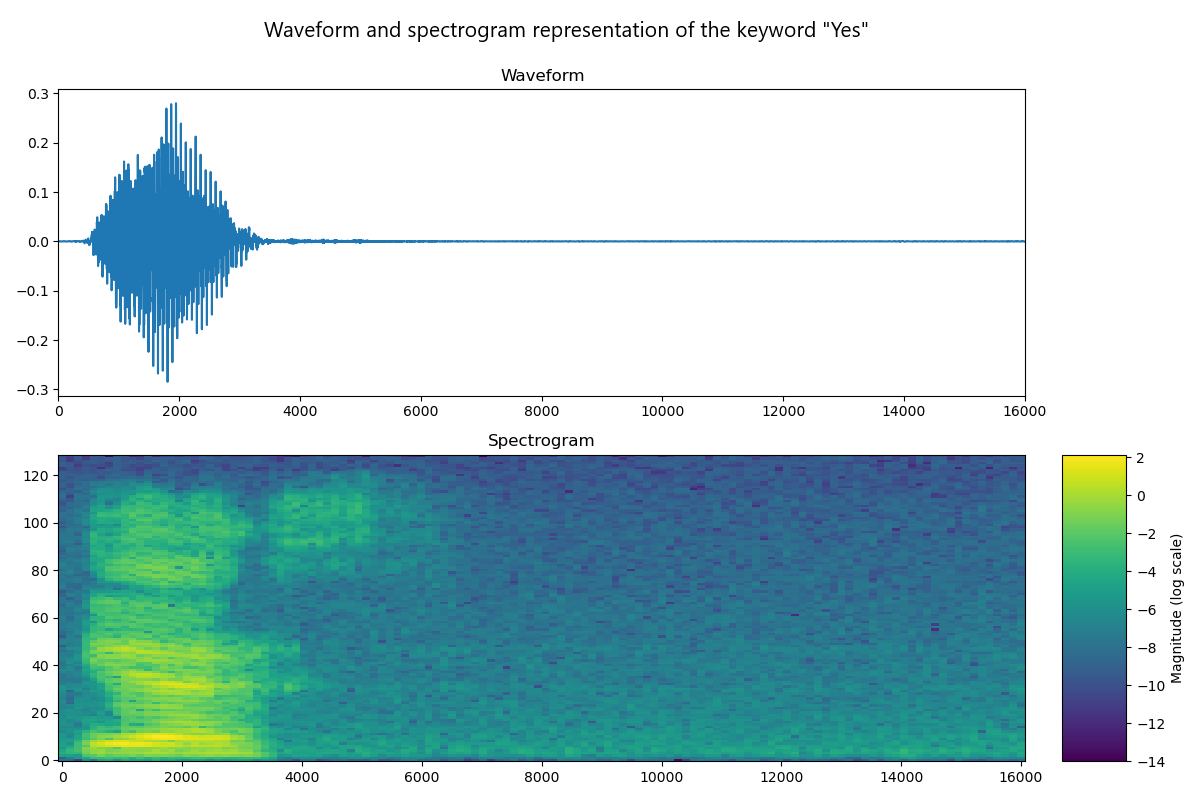
\includegraphics[width=0.8\textwidth]{Images/Results/audioWaveSpectrogramYes}
	\caption{Waveform and spectrogram representation of the keyword "yes"} \label{fig:audioWaveSpectrogramYes}
\end{figure}

\section{Model Export and Conversion}

The trained model was successfully exported, and a saved model was created. Furthermore, the saved model was converted to TensorFlow Lite format (TFLite) for deployment on resource-constrained platforms.


\section{Model Training and Performance}

The training process commenced, lasting approximately 22 seconds per epoch. The model exhibited an improvement in performance over the course of the epochs, as evident in the training and validation metrics.

\section{Epoch-wise Performance}

The epoch-wise performance evaluations are shown in Figure \ref{fig:trainingProgress}.

\begin{itemize}
	\item \textbf{Epochs 1-5: Initial Training Progress}
	\begin{itemize}
		\item The initial training phase demonstrates notable progress as the model rapidly enhances its performance.
		\item Epoch 1 starts with a loss of 1.7081 and an accuracy of 39.48\%. This suggests an initial grasp of data patterns by the model.
		\item Subsequent epochs show consistent improvement, reaching a training accuracy of 79.50\% by Epoch 5. The corresponding loss decreases from 1.7081 to 0.5908, indicating effective learning.
		\item The training time per epoch varies between 7 and 13 seconds, showcasing moderate efficiency.
	\end{itemize}
	
	\item \textbf{Epochs 6-10: Continued Improvement and Stability}
	\begin{itemize}
		\item The model continues to refine its features, achieving a peak training accuracy of 89.39\% by Epoch 10.
		\item The loss further decreases to 0.3241, demonstrating the model's ability to generalize well on the training data.
		\item The stability in training time per epoch (7-8 seconds) indicates consistent computational efficiency during this phase.
	\end{itemize}
	
	\item \textbf{Validation Results after 10 Epochs}
	\begin{itemize}
		\item The model exhibits strong generalization to unseen data with a validation accuracy of 86.12\% after 10 epochs.
		\item The validation loss of 0.4351 is slightly lower than the training loss, indicating a good level of generalization without overfitting.
		\item The low inference time (2 milliseconds per step) suggests that the trained model is computationally efficient during the testing phase.
	\end{itemize}
\end{itemize}

\begin{figure}[h!]
	\centering
	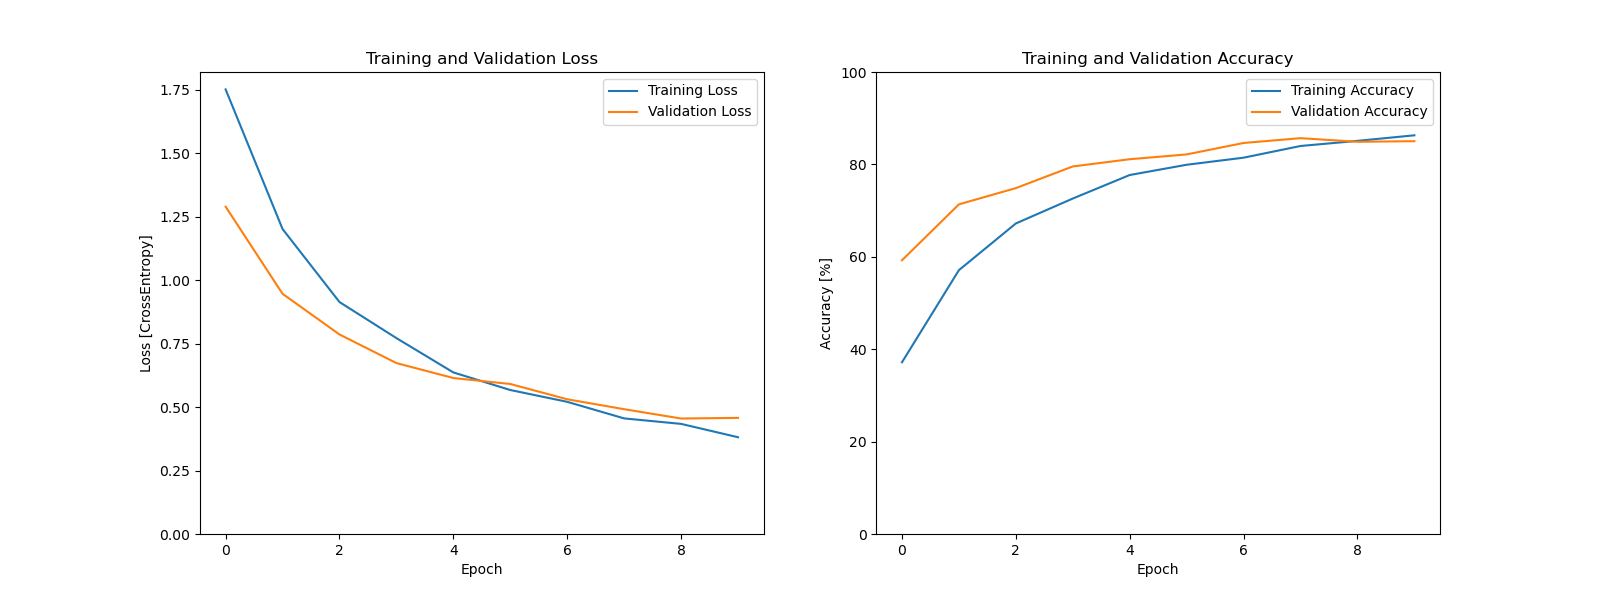
\includegraphics[width=0.8\textwidth]{Images/Results/trainingProgress}
	\caption{Epoch-wise performance evaluation of the CNN model} \label{fig:trainingProgress}
\end{figure}

\subsection{Test Dataset Evaluation}

The result of this evaluation was a test accuracy of 85\%. This indicates that the model correctly classified 85\% portion of the samples.

\section{Arduino Nano 33 BLE Sense Results}

The board shows relatively accurate responses when prompted with the designated keyword spoken within a 20cm range. At a distance longer than 20cm, it normally doesn't show a response. However, there are instances where the board may fail to register a response even within a 20cm range. In addition, it may occasionally misinterpret a "yes" or "no" keyword, classifying it as an unknown keyword, which is signified by the activation of a blue LED. Moreover, environmental noise can contribute to the occurrence of unknown keyword responses on the board. While generally reliable, these occasional anomalies highlight the sensitivity of the system to external factors. The board's responses are shown in the Figure \ref{fig:ArduinoImages}.

\begin{figure}[h!]
	\centering
	
	\begin{subfigure}{0.3\textwidth}
		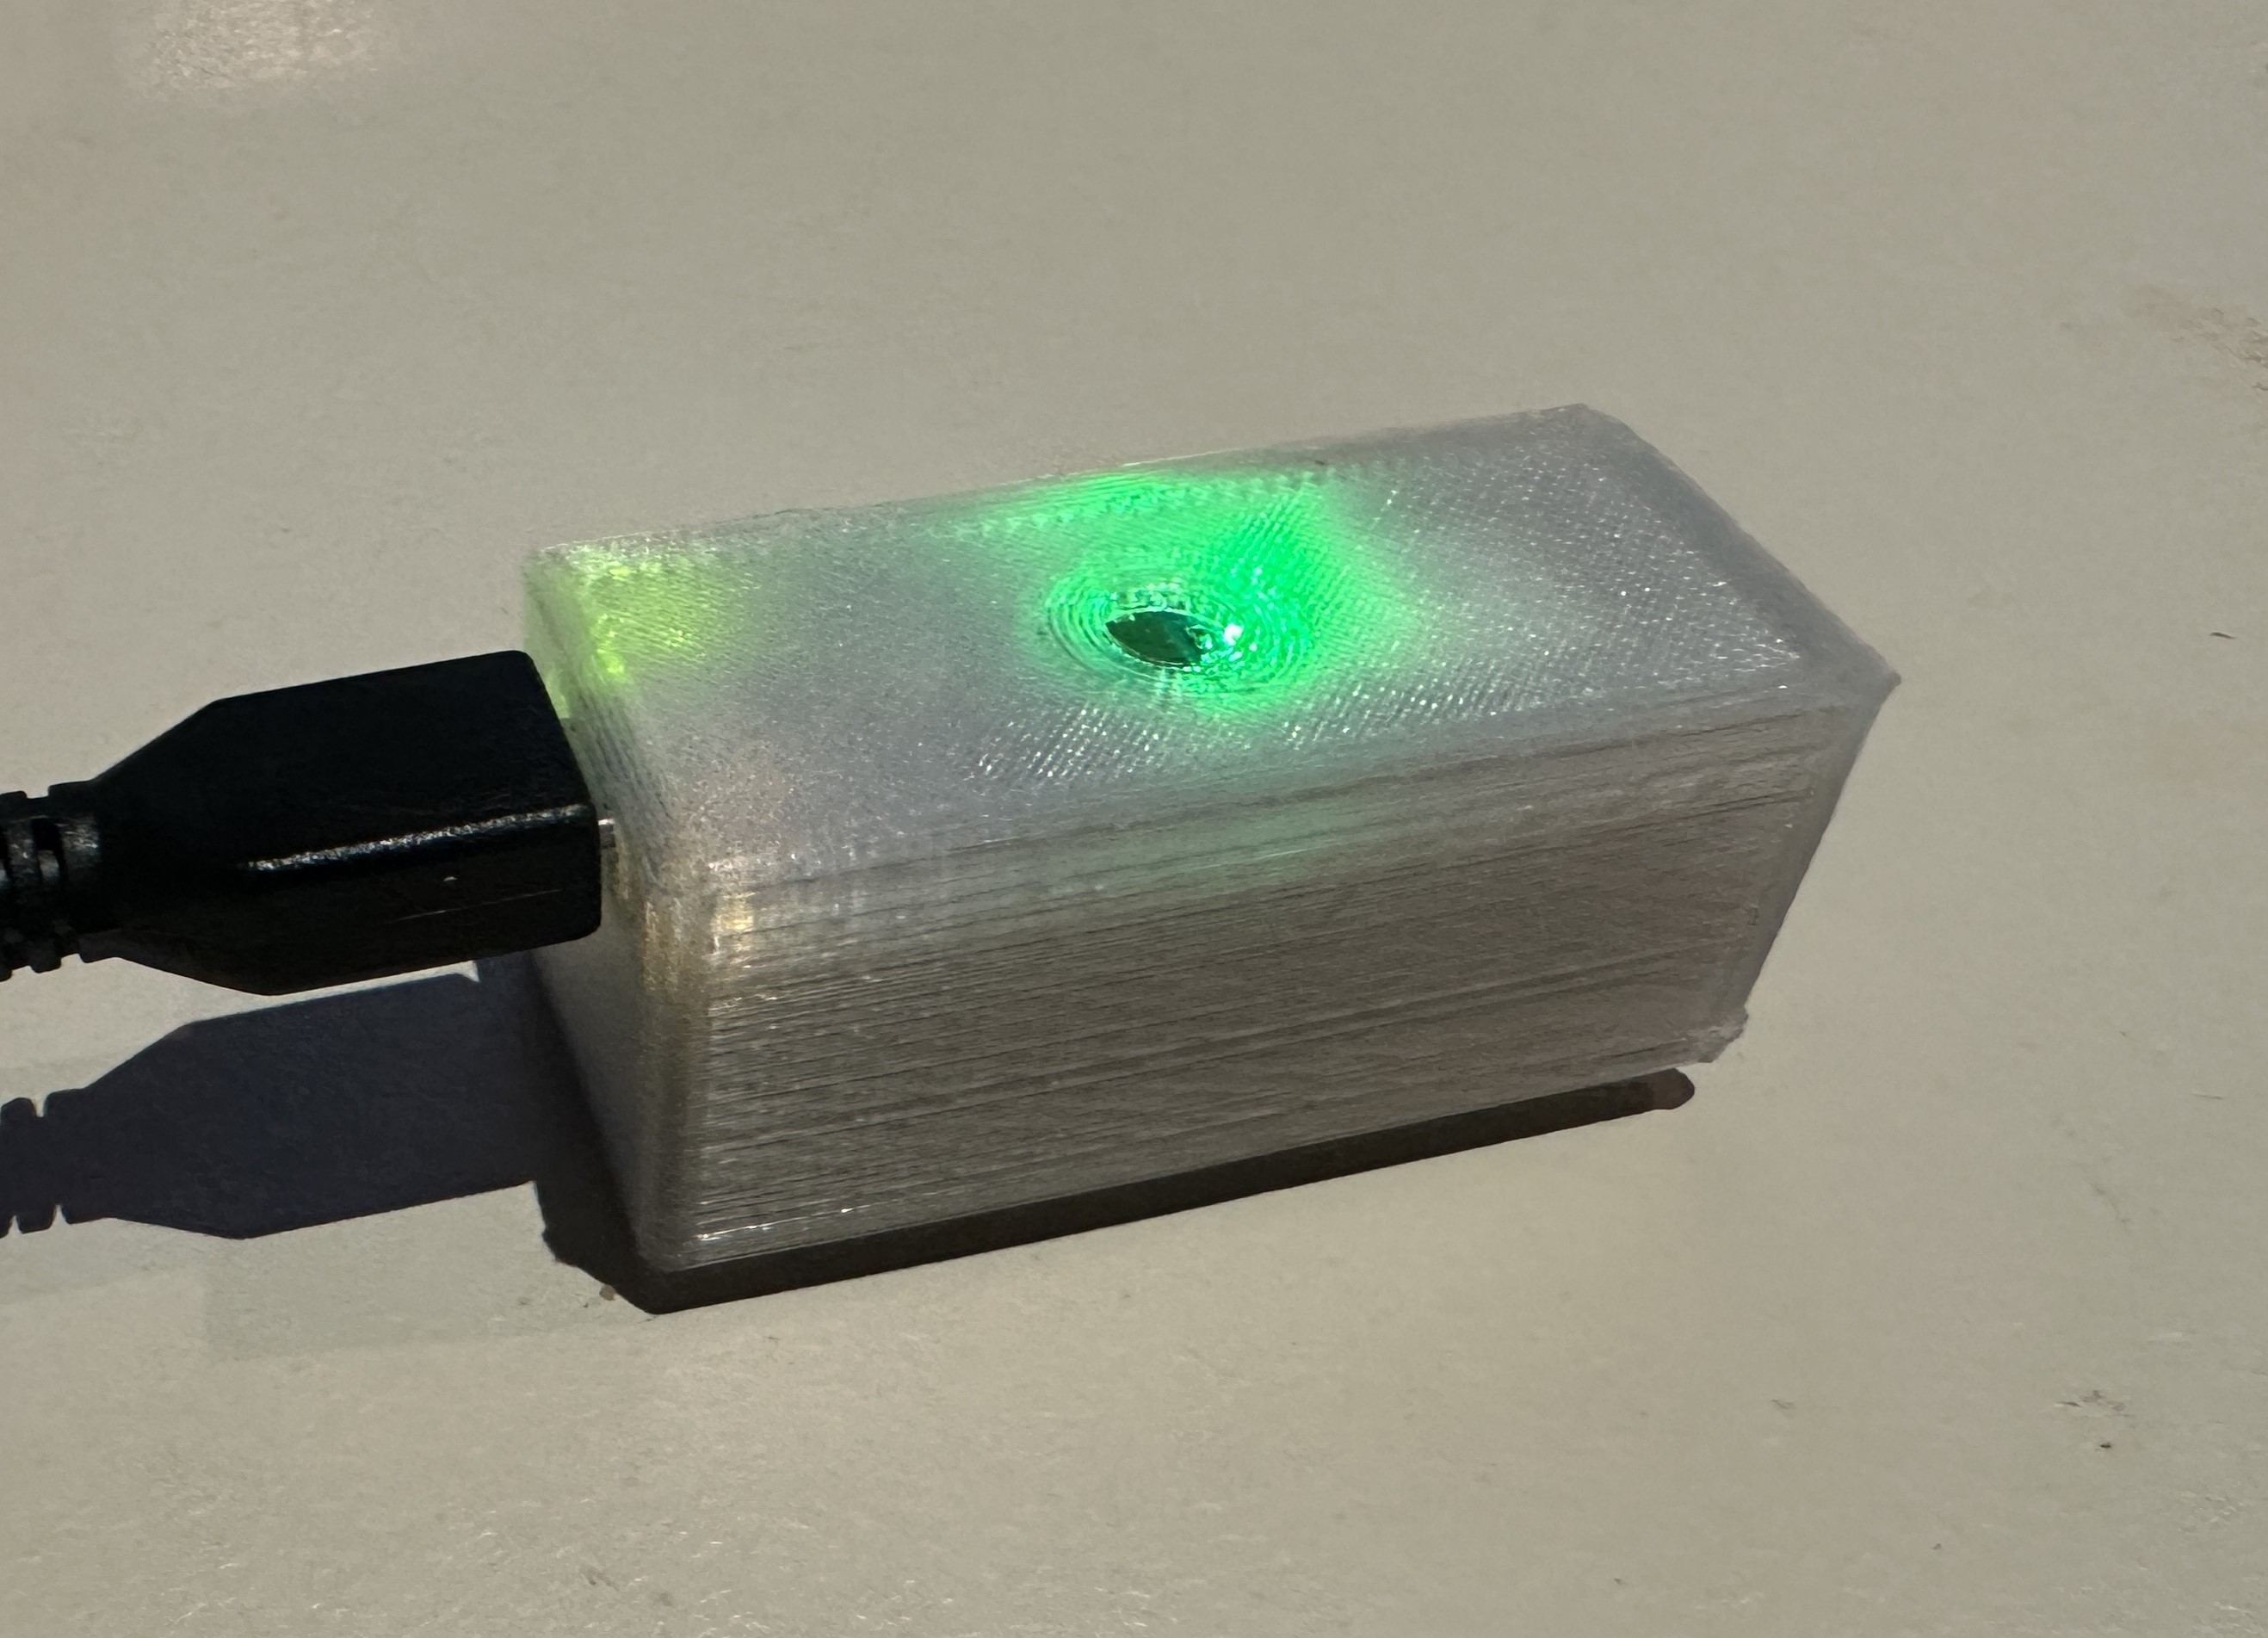
\includegraphics[width=\linewidth]{Images/Results/ArduinoGreen}
		\caption{}    % \caption{} is kept to keep (a), (b), (c) etc. below each subfigure.
		\label{subfig:ArduinoGreen}
	\end{subfigure}
	\hfill
	\begin{subfigure}{0.3\textwidth}
		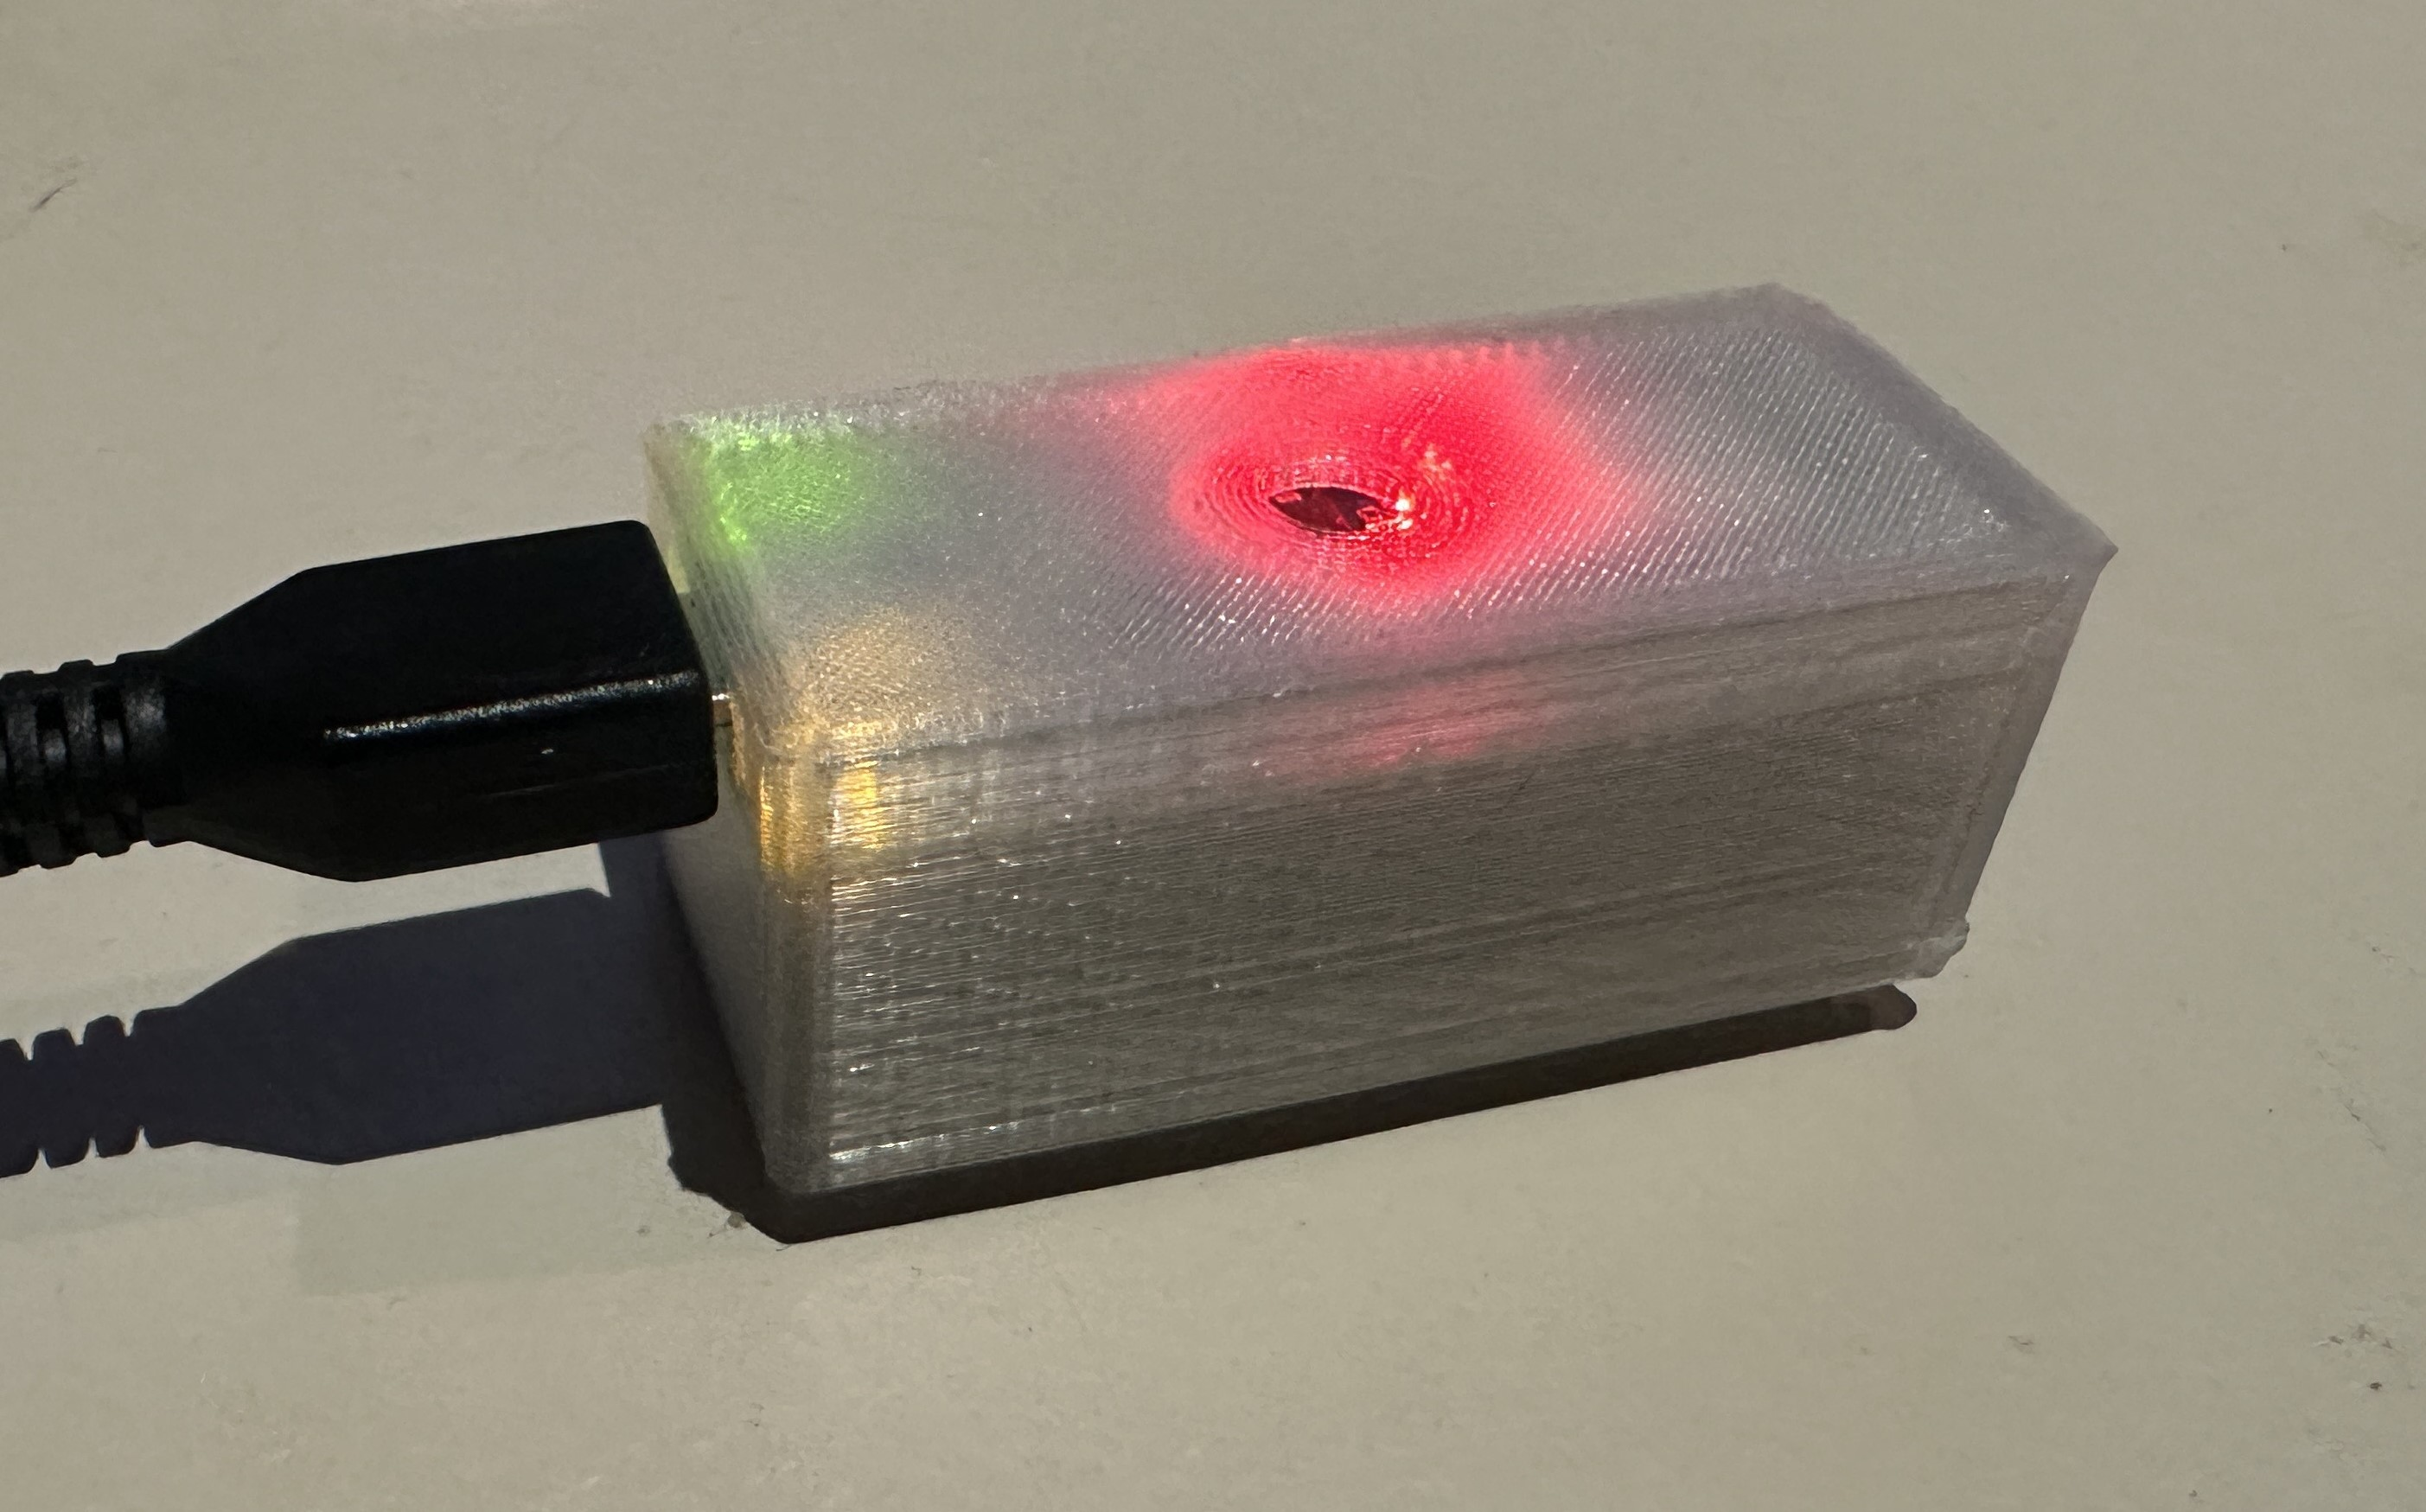
\includegraphics[width=\linewidth]{Images/Results/ArduinoRed}
		\caption{}    % \caption{} is kept to keep (a), (b), (c) etc. below each subfigure.
		\label{subfig:ArduinoRed}
	\end{subfigure}
	\hfill
	\begin{subfigure}{0.3\textwidth}
		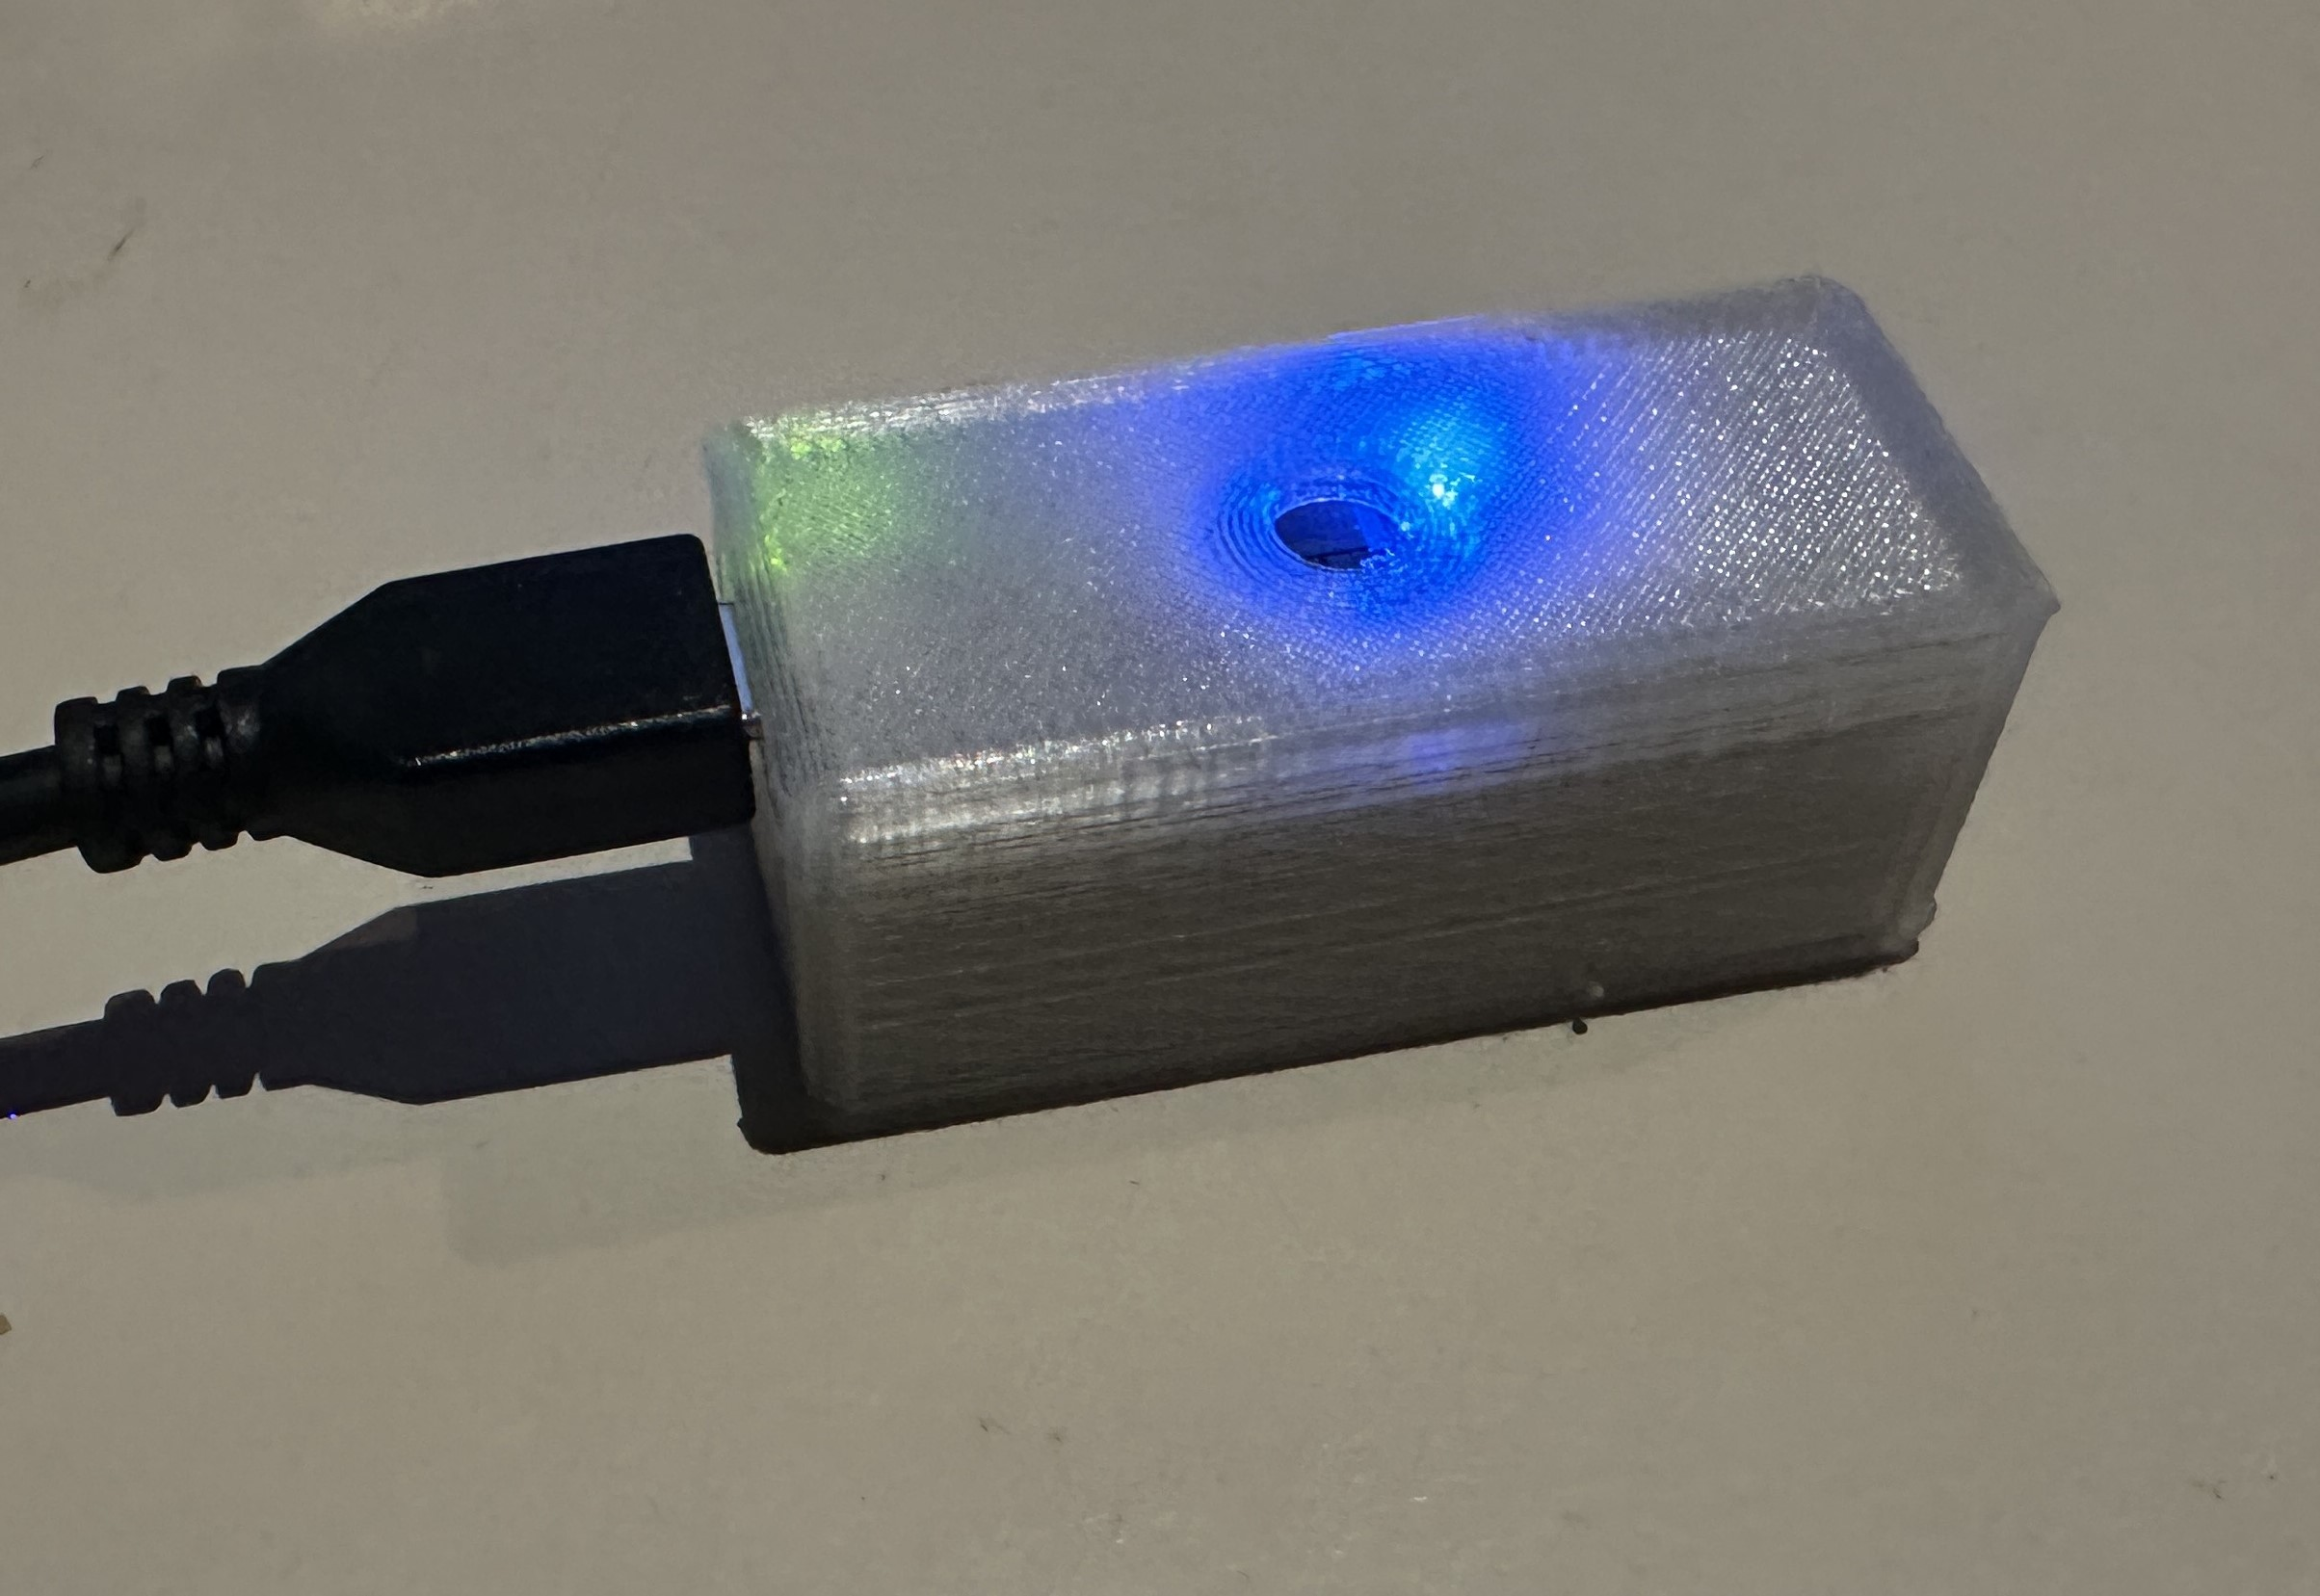
\includegraphics[width=\linewidth]{Images/Results/ArduinoBlue}
		\caption{}    % \caption{} is kept to keep (a), (b), (c) etc. below each subfigure.
		\label{subfig:ArduinoBlue}
	\end{subfigure}
	
	\caption{Board response: (\subref{subfig:ArduinoGreen}) Response to the keyword "yes" (\subref{subfig:ArduinoRed}) Response to the keyword "no" (\subref{subfig:ArduinoBlue}) Response to unknown keyword}
	\label{fig:ArduinoImages}
\end{figure}







